% ----------------------------------------------------------
%% Capitulo3-MetodosNumericos.tex 
% ----------------------------------------------------------
% Metodos Numericos
% ----------------------------------------------------------
\chapter[Métodos]{Métodos Numéricos}
\label{Cap_MetodosNumericos}

Neste capítulo, descrevem-se os métodos numéricos adotados para resolver as equações bidimensionais que governam o escoamento de fluidos viscoelásticos incompressíveis, formuladas em termos da Formulação Vorticidade-Função de Corrente. Utiliza-se a discretização espacial de alta ordem, baseada em esquemas compactos de diferenças finitas, e um método de integração temporal eficiente. A abordagem escolhida visa garantir elevada precisão e estabilidade, essenciais para a solução de problemas envolvendo complexidade como os escoamentos viscoelásticos.

\section{Método para discretização temporal}\label{SecDiscretizacaoTemporal}

Para realizar o avanço temporal, envolvendo as Equações \eqref{eq_conservacao_momentum_nao_newtoniano_admensional} e \eqref{eq_tensores_lpog_admensional}, utiliza-se o método de Runge-Kutta de quarta ordem de precisão \cite{ferziger2002computational}. Neste estudo, empregamos o método Previsor-Corretor, onde os passos de Euler explícito e implícito são utilizados como previsor e corretor, respectivamente, para avançar o sistema do tempo $t$ para o tempo $t + \Delta t / 2$. Posteriormente, o sistema é avançado para o tempo $t + \Delta t$ com um previsor baseado na regra do ponto médio e um corretor usando a regra de Simpson. Os quatro passos do método são descritos pelas seguintes equações:
\begin{gather}
    \begin{aligned}
        &\textbf{1º passo:}& \hspace{0.3cm}\varphi^{\left(n+\frac{1}{2}\right)^{*}} &= \varphi^n+\frac{\Delta t}{2} g_{\varphi}\left(t^n, \varphi^n\right),\\
        &\textbf{2º passo:}& \hspace{0.3cm}\varphi^{\left(n+\frac{1}{2}\right)^{* *}} &= \varphi^n+\frac{\Delta t}{2} g_{\varphi}\left(t^{n+\frac{1}{2}}, \varphi^{\left(n+\frac{1}{2}\right)^*}\right),\\
        &\textbf{3º passo:}& \hspace{0.3cm}\varphi^{(n+1)^*} &= \varphi^n+\Delta t g_{\varphi}\left(t^{n+\frac{1}{2}},\varphi^{\left(n+\frac{1}{2}\right)^{* *}}\right),\\
        &\textbf{4º passo:}& \hspace{0.3cm}\varphi^{n+1} &= \varphi^n+\frac{\Delta t}{6}\bigg[g_{\varphi}\left(t^n, \varphi^n\right) + 2 g_{\varphi}\left(t^{n+\frac{1}{2}}, \varphi^{\left(n+\frac{1}{2}\right)^{*}}\right) + \\
        & & & ~~~ + 2 g_{\varphi}\left(t^{n+\frac{1}{2}}, \varphi_{z}^{\left(n+\frac{1}{2}\right)^{**}}\right)+ g_{\varphi}\left(t^{n+1}, \varphi^{(n+1)^{*}}\right)\bigg].\label{eq_rk_4order}
    \end{aligned}
\end{gather}

Nos passos do método de Runge-Kutta descritos na \autoref{eq_rk_4order}, a variável $\varphi$ pode representar qualquer uma das funções $\omega_{z}$, $T_{xx}$, $T_{xy}$ ou $T_{yy}$. Para a vorticidade $\omega_{z}$, a expressão de $g_{\omega_{z}}(t, \omega_{z})$ é dada como segue:
\begin{gather}
    \begin{aligned}
        g_{\omega_{z}}\left(t, \omega_z\right) = &~- u\frac{\partial\left(\omega_{z}\right)}{\partial x} - v \frac{\partial\left(\omega_{z}\right)}{\partial y} + \frac{\beta_{nn}}{R e}\left(\frac{\partial^2 \omega_{z}}{\partial x^2} + \frac{\partial^2 \omega_{z}}{\partial y^2}\right) + \frac{\partial^2 T_{x x}}{\partial x \partial y} + \frac{\partial^2 T_{x y}}{\partial y^2} - \\ &~- \frac{\partial^2 T_{x y}}{\partial x^2} - \frac{\partial^2 T_{y y}}{\partial x \partial y},
    \end{aligned}
\end{gather}
Para os tensores $T_{xx}$, $T_{xy}$ e $T_{yy}$, as expressões correspondentes são as seguintes:
\begin{subequations}
\begin{align}
    g_{T_{xx}}\left(t, T_{xx}\right) & = - \frac{f_{tr}(\mathbf{T})T_{xx}}{\operatorname{Wi}} - \left[\frac{\partial (uT_{xx})}{\partial x} + \frac{\partial (vT_{xx})}{\partial y} - 2T_{xx}\frac{\partial u}{\partial x} - 2T_{xy}\frac{\partial u}{\partial y}\right] - \frac{\alpha_{G}\operatorname{Re}}{1-\beta_{nn}}\left(T_{xx}^{2} + T_{xy}^{2}\right) - \nonumber \\ & - \xi\left(2T_{xx}\frac{\partial u}{\partial x} + T_{xy}\left(\frac{\partial u}{\partial y} + \frac{\partial v}{\partial x}\right)\right) + \frac{2(1-\beta_{nn})}{\operatorname{Wi}\operatorname{Re}}\frac{\partial u}{\partial x},\label{eq_gies_txx_steps_rk}\\[7mm]
    g_{T_{xy}}\left(t, T_{xy}\right) & = - \frac{f_{tr}(\mathbf{T})T_{xy}}{\operatorname{Wi}} - \left[\frac{\partial (uT_{xy})} {\partial x} + \frac{\partial (vT_{xy})}{\partial y} - T_{xx}\frac{\partial v}{\partial x} - T_{yy}\frac{\partial u}{\partial y}\right] - \frac{\alpha_{G}\operatorname{Re}}{1-\beta_{nn}}\left[T_{xy}\left(T_{xx} + T_{yy}\right)\right] - \nonumber \\ & - \frac{\xi}{2}\left(T_{xx} + T_{yy}\right)\left(\frac{\partial u}{\partial y} + \frac{\partial v}{\partial x}\right) + \frac{(1-\beta_{nn})}{\operatorname{Wi}\operatorname{Re}}\left(\frac{\partial v}{\partial x} + \frac{\partial u}{\partial y}\right),\label{eq_gies_txy_steps_rk}\\[7mm]
    g_{T_{yy}}\left(t, T_{yy}\right) & = - \frac{f_{tr}(\mathbf{T})T_{yy}}{\operatorname{Wi}} - \left[\frac{\partial (uT_{yy})}{\partial x} + \frac{\partial (vT_{yy})}{\partial y} - 2T_{xy}\frac{\partial v}{\partial x} - 2T_{yy}\frac{\partial v}{\partial y}\right] - \frac{\alpha_{G}\operatorname{Re}}{1-\beta_{nn}}\left(T_{xy}^{2} + T_{yy}^{2}\right) - \nonumber \\ & - \xi\left(2T_{yy}\frac{\partial v}{\partial y} + T_{xy}\left(\frac{\partial u}{\partial y} + \frac{\partial v}{\partial x}\right)\right) + \frac{2(1-\beta_{nn})}{\operatorname{Wi}\operatorname{Re}}\frac{\partial v}{\partial y}.\label{eq_gies_tyy_steps_rk}
\end{align}
\end{subequations}

\section{Método para discretização espacial}\label{Sec_Metodos_Numericos_Discretizacao_Espacial}

Para o cálculo das derivadas espaciais, a discretização das derivadas foi realizada utilizando esquemas de diferenças finitas compactas conforme apresentado por \citeonline{souza2003}. Estes esquemas garantem precisão de quarta ordem tanto para as derivadas de primeira quanto de segunda ordem. Para simplificar a nomenclatura e a implementação dos métodos, as formulações são apresentadas em uma dimensão (1D), embora sejam aplicadas posteriormente para problemas bidimensionais. Ao aplicar esses esquemas para aproximar as derivadas de primeira e segunda ordem de uma função $f$, é necessário resolver sistemas lineares tridiagonais.

Para a derivada espacial de primeira ordem nos pontos de fronteira, utilizamos uma aproximação a jusante de quarta ordem, que assegura uma alta precisão ao tratar os efeitos da fronteira. Nos pontos de fronteira, a fórmula de quarta ordem é expressa como:
\begin{equation}
    f_1^{\prime}+3 f_2^{\prime}=\frac{1}{ 6h}\left(-17f_1 + 9f_2 + 9f_3 - f_4 \right)+O\left(h^4\right)
\end{equation}
ou
\begin{equation}
    f_n^{\prime} + 3f_{n-1}^{\prime} = -\frac{1}{ 6h}\left(-17f_{n} + 9f_{n-1} + 9f_{n-2} - f_{n-4} \right)+O\left(h^4\right),
\end{equation}
e nos pontos centrais a aproximação de quarta ordem usada é dada por:
\begin{equation}
    f_{i-1}^{\prime}+4 f_i^{\prime}+f_{i+1}^{\prime}=\frac{3}{ h}\left(f_{i+1}-f_{i-1}\right) +O\left(h^4\right).
\end{equation}

A implementação desses esquemas para todas as derivadas requer a resolução de sistemas lineares tridiagonais. A matriz associada a esse sistema pode ser expressa da seguinte forma:
\begin{equation}
\left[\begin{array}{ccccccc}
1 & 3 & & & & & \\
1 & 4 & 1 & & & & \\
& & \ddots & & & & \\
& & 1 & 4 & 1 & & \\
& & & & \ddots & & \\
& & & & 1 & 4 & 1 \\
& & & & & 3 & 1
\end{array}\right]\left[\begin{array}{c}
f_1^{\prime} \\
f_2^{\prime} \\
\vdots \\
f_i^{\prime} \\
\vdots \\
f_{n-1}^{\prime} \\
f_n^{\prime}
\end{array}\right] \approx \frac{1}{h}\left[\begin{array}{c}\frac{1}{6}\left(-17f_1 + 9f_2 + 9f_3 - f_4 \right) \\ 3(f_3 - f_1) \\ \vdots \\ 3\left(f_{i+1}-f_{i-1}\right) \\ \vdots \\ 3\left(f_{n}-f_{n-2}\right) \\ \frac{1}{6}\left(-17f_n + 9f_{n-1} + 9f_{n-2} - f_{n-3}\right)\end{array}\right].
\end{equation}

Para a derivada de segunda ordem, também foi utilizado um esquema de quarta ordem. Nos pontos de fronteira, aproxima a derivada de segunda ordem como segue:
\begin{equation}
    f_1^{\prime \prime} + 11f_{2}^{\prime \prime} = \frac{1}{3h^{2}}\left(39f_{1} - 81f_{2} + 45f_{3} - 3f_{4}\right)+O\left(h^4\right)
\end{equation}
ou
\begin{equation}
    f_{n}^{\prime \prime} + 11f_{n-1}^{\prime \prime} = -\frac{1}{3h^{2}}\left(39f_{n} - 81f_{n-1} + 45f_{n-2} - 3f_{n-3}\right)+O\left(h^4\right),
\end{equation}
e nos pontos centrais a aproximação de quarta ordem usada é dada por:
\begin{equation}
    1 f_{i-1}^{\prime \prime}+10 f_i^{\prime \prime}+1 f_{i+1}^{\prime \prime}=\frac{1}{ h^2}12\left(f_{i-1} + f_{i+1}\right) -24f_{i}+O\left(h^4\right) .
\end{equation}

Da mesma forma que no caso das derivadas de primeira ordem, é necessário resolver um sistema linear tridiagonal, cuja matriz pode ser expressa como:
\begin{equation}
\left[\begin{array}{ccccccc}
1 & 11 & & & & & \\
1 & 10 & 1 & & & & \\
& & \ddots & & & & \\
& & 1 & 10 & 1 & & \\
& & & & \ddots & & \\
& & & & 1 & 10 & 1 \\
& & & & & 11 & 1
\end{array}\right]\left[\begin{array}{c}
f_1^{\prime \prime} \\
f_2^{\prime \prime} \\
\vdots \\
f_i^{\prime \prime} \\
\vdots \\
f_{n-1}^{\prime \prime} \\
f_n^{\prime \prime}
\end{array}\right] \approx \frac{1}{h^2}\left[\begin{array}{c}\frac{1}{3}\left(39f_1 - 81f_2 + 45f_3 - 3f_4\right) \\ 12\left(f_1 + f_3\right) -24f_2 \\ \vdots \\ 12\left(f_{i-1} + f_{i+1}\right) -24f_{i} \\ \vdots \\ 12\left(f_{n-2} + f_{n}\right) -24f_{n-1}  \\ -\frac{1}{3}\left(39f_{n} - 81f_{n-1} + 45f_{n-2} - 3f_{n-3}\right)\end{array}\right].
\end{equation}

Embora as equações tenham sido apresentadas para uma dimensão, a simplicidade da notação e a estrutura das equações permitem sua aplicação direta a problemas bidimensionais (2D). Para isso, as derivadas em $x$ e $y$ são tratadas separadamente, utilizando esquemas semelhantes para cada direção. Essa abordagem mantém a precisão de quarta ordem nas discretizações espaciais e facilita a implementação dos esquemas numéricos.

\section{Solução Numérica da Equação de Poisson}

Para solução numérica da equação de Poisson, advinda da formulação Vorticidade-Função de Corrente, adotadou-se um método iterativo \textit{Multigrid} do tipo Esquema de Aproximação Total (FAS, do inglês: \textit{Full Aproximation Scheme})\sigla*{FAS}{Full Aproximation Scheme}. O método multigrid é uma técnica amplamente utilizada para resolver equações diferenciais parciais, particularmente as de natureza elíptica, pois ele acelera a convergência dos métodos iterativos tradicionais, utilizando várias resoluções da malha (ou \textit{grids}) para eliminar erros em diferentes escalas. Um dos principais benefícios desse método é sua capacidade de combinar a alta precisão de malhas refinadas com a eficiência de malhas mais grosseiras. 

O sistema linear é resolvido por meio de um ciclo \textit{multigrid} do tipo V, com quatro níveis de malha. A escolha de um fator de engrossamento igual a 2 foi fundamentada nos estudos de \citeonline{brandt1977multi}, que demonstram que esta relação oferece um bom equilíbrio entre eficiência e precisão. O método de SOR \sigla*{SOR}{\textit{Sucessive Over-Relaxation}} é empregado, com a técnica de Gauss-Seidel aplicada após o prolongamento. Além disso, o fator de relaxação $r_2$ é utilizado nos casos apropriados para acelerar a convergência. O processo se inicia na malha com o menor espaçamento $h$, onde são realizadas $N_1$ iterações utilizando o método SOR para aproximar a solução da equação de Poisson:
$$
\nabla^2 v_h=s_h .
$$

Após estas iterações, o resíduo $d_h$ é calculado, representando a diferença entre o termo fonte $s_h$ e o operador aplicado à solução aproximada $v_h$:
$$
d_h=s_h-\nabla^2 v_h .
$$

O resíduo $d_h$ é então transferido da malha refinada ($h$) para uma malha menos refinada ($2h$) por meio de uma operação de restrição. Nesta etapa, utiliza-se a técnica de ponderação total (FW, do inglês: \textit{Full Weighting}) para transferir o resíduo, enquanto a solução $v_h$ é transmitida diretamente para a malha $2h$ através de injeção direta (SI, do inglês: \textit{Straight Injection}):
$$
\begin{aligned}
&v_h \Rightarrow v_{2 h} \quad(SI), \\
&d_h \Rightarrow d_{2 h} \quad(FW) .
\end{aligned}
$$
Com os valores transferidos, o termo fonte na nova malha $2h$ é atualizado:
$$
s_{2 h} = d_{2 h}+\nabla^2 v_{2 h} .
$$
Novamente, são realizadas $N_1$ iterações nesta malha para resolver a equação:
$$
\nabla^2 v_{2 h} = s_{2 h} .
$$

Após resolver a equação na malha $2h$, calcula-se o resíduo $d_{2h}$ e aplica-se uma correção. O valor da correção é então interpolado de volta para a malha refinada ($h$) utilizando interpolação bilinear, conforme ilustrado na \autoref{fig_multigrid_interpolacao_bilinear}:
\[
\begin{aligned}
\operatorname{corr}_{8h} &\Rightarrow \operatorname{corr}_{4h}, \\
v_{4h} &\Leftarrow v_{4h} + \operatorname{corr}_{4h}.
\end{aligned}
\]
\begin{figure}[htb]
    \centering 
    \caption{Interpolação Bilinear utilizado no método \textit{Multigrid}}\label{fig_multigrid_interpolacao_bilinear} 
    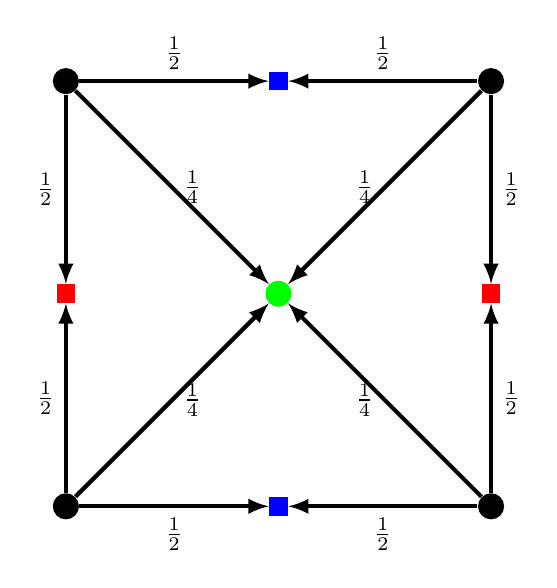
\begin{tikzpicture}[scale=0.9]
        % Define os nos
        \node[circle,fill=black] (A) at (0,6) {};
        \node[circle,fill=black] (B) at (6,6) {};
        \node[circle,fill=black] (C) at (6,0) {};
        \node[circle,fill=black] (D) at (0,0) {};
        \node[rectangle,fill=blue] (E) at (3,6) {};
        \node[rectangle,fill=blue] (F) at (3,0) {};
        \node[rectangle,fill=red] (G) at (0,3) {};
        \node[rectangle,fill=red] (H) at (6,3) {};
        \node[circle,fill=green] (I) at (3,3) {};
        % Conecta nos
        \draw[->, thick, >=latex, line width=1.5pt] (A) -- node[above] {$\frac{1}{2}$} (E);
        \draw[->, thick, >=latex, line width=1.5pt] (B) -- node[above] {$\frac{1}{2}$} (E);
        \draw[->, thick, >=latex, line width=1.5pt] (B) -- node[right] {$\frac{1}{2}$} (H);
        \draw[->, thick, >=latex, line width=1.5pt] (C) -- node[right] {$\frac{1}{2}$} (H);
        \draw[->, thick, >=latex, line width=1.5pt] (C) -- node[below] {$\frac{1}{2}$} (F);
        \draw[->, thick, >=latex, line width=1.5pt] (D) -- node[below] {$\frac{1}{2}$} (F);
        \draw[->, thick, >=latex, line width=1.5pt] (D) -- node[left]  {$\frac{1}{2}$} (G);
        \draw[->, thick, >=latex, line width=1.5pt] (A) -- node[left]  {$\frac{1}{2}$} (G);
        \draw[->, thick, >=latex, line width=1.5pt] (A) -- node[right] {$\frac{1}{4}$} (I);
        \draw[->, thick, >=latex, line width=1.5pt] (B) -- node[left]  {$\frac{1}{4}$} (I);
        \draw[->, thick, >=latex, line width=1.5pt] (C) -- node[left]  {$\frac{1}{4}$} (I);
        \draw[->, thick, >=latex, line width=1.5pt] (D) -- node[right] {$\frac{1}{4}$} (I);
    \end{tikzpicture}
    \fadaptada{rogenski2011desenvolvimento}
\end{figure}

Na malha $4h$, realiza-se mais uma série de $N_3$ iterações utilizando o método de Gauss-Seidel, resolvendo a equação:
\[
\nabla^2 v_{4h} = s_{4h}.
\]
O ciclo multigrid é finalizado após aplicar uma nova interpolação bilinear e corrigir os valores na malha $2h$, como mostrado na \autoref{fig_multigrid_cicle_v}. O número de ciclos repetidos depende da tolerância de erro especificada para o resíduo final na malha refinada. O algoritmo continua até que o erro residual seja inferior ao valor de tolerância definido.

\begin{figure}[htb]
    \centering
    \caption{Esquema do ciclo V no método multigrid FAS.}\label{fig_multigrid_cicle_v}
    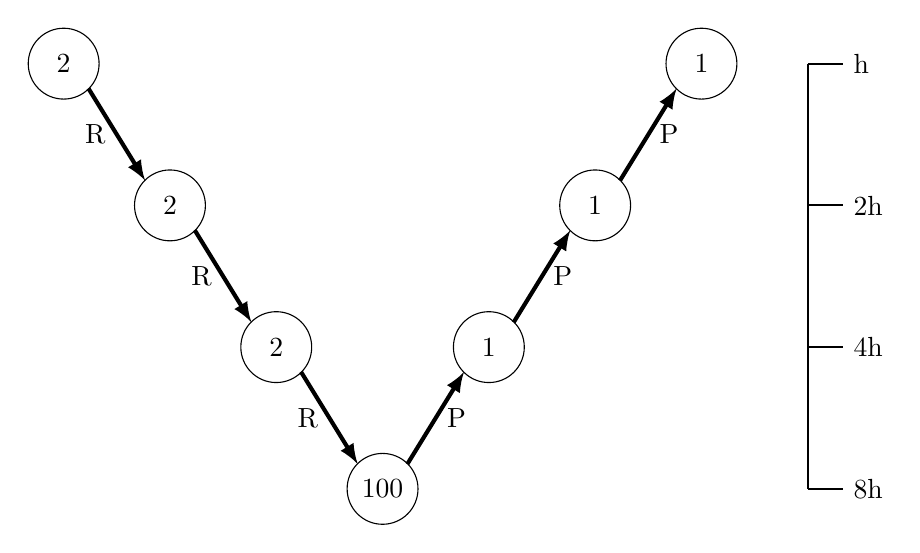
\begin{tikzpicture}[scale=0.9]
        \draw (0,8) circle (0.5) node {2};
        \draw (1.5,6) circle (0.5) node {2};
        \draw (3,4) circle (0.5) node {2};
        \draw (4.5,2) circle (0.5) node {100};
        \draw (6,4) circle (0.5) node {1};
        \draw (7.5,6) circle (0.5) node {1};
        \draw (9,8) circle (0.5) node {1};
        \draw[->, thick, >=latex, line width=1.5pt] (0.35,7.65) -- (1.15,6.35) node[midway,left] {R};
        \draw[->, thick, >=latex, line width=1.5pt] (1.85,5.65) -- (2.65,4.35) node[midway,left] {R};
        \draw[->, thick, >=latex, line width=1.5pt] (3.35,3.65) -- (4.15,2.35) node[midway,left] {R};
        \draw[->, thick, >=latex, line width=1.5pt] (7.85,6.35) -- (8.65,7.65) node[midway,right] {P};
        \draw[->, thick, >=latex, line width=1.5pt] (6.35,4.35) -- (7.15,5.65) node[midway,right] {P};
        \draw[->, thick, >=latex, line width=1.5pt] (4.85,2.35) -- (5.65,3.65) node[midway,right] {P};
        \draw[thick] (10.5,8) -- (10.5,2);
        \draw[thick] (10.5,8) -- (11,8) node[right] {h};
        \draw[thick] (10.5,6) -- (11,6) node[right] {2h};
        \draw[thick] (10.5,4) -- (11,4) node[right] {4h};
        \draw[thick] (10.5,2) -- (11,2) node[right] {8h};
    \end{tikzpicture}
    \fadaptada{rogenski2011desenvolvimento}
\end{figure}

O método multigrid destaca-se por sua eficácia em acelerar a convergência de soluções numéricas para equações diferenciais parciais, especialmente em problemas elípticos, como a equação de Poisson. A abordagem multiescala, que combina malhas refinadas e grosseiras, permite corrigir os erros em diferentes escalas, resultando em uma solução rápida e precisa.

Para todos os casos considerados, $N_3=1$. O número de ciclos necessário para que a solução da equação seja, de fato, obtida, está associado ao resíduo obtido na malha mais fina. Se o valor obtido for menor do que uma dada tolerância de referência, o algoritmo é finalizado.

\section{Método de filtragem}\label{SecFiltragem}

Adotou-se também a estratégia de se realizar filtragem espacial baseada em \cite{lele1992compact}. Dentre os diversos métodos compactos de filtragem propostos pelo autor, opta-se pelo uso de um método compacto tridiagonal de até sexta ordem de precisão. A filtragem é aplicada ao final de cada iteração temporal e consiste em recalcular a distribuição dos componentes de vorticidade por meio de um sistema, no caso:
\begin{align}
\left[\begin{array}{ccccccccccc}
1 &  & & & & & & & & &\\
 & 1 &  & & & & & & & & \\
& & 1 & & & & & & & &\\
& &  & . & . & .&  &  & & & \\
& & &  & \alpha & 1 & \alpha &  & & &  \\
& & & &  & . & . & . &  & & \\
& & & & &  &  & & 1 & & \\
& & & & &  &  & & & 1 & \\
& & & & &  &  & & &  & 1
\end{array}\right] \left[\begin{array}{c}
\varphi_{z1} \\
\varphi_{z2}  \\
\varphi_{z3}  \\
 . \\
\varphi_{zi}  \\
 . \\
\varphi_{zimax-2} \\
\varphi_{zimax-1} \\
\varphi_{zimax} 
\end{array}\right] = \hspace{1cm} \nonumber\\ 
=\left[\begin{array}{c}
(15\varphi_{z1}^* +  4 \varphi_{z2}^* -  6 \varphi_{z3}^* +  4  \varphi_{z4}^*
 -         \varphi_{z5}^* ) / 16 \\
( \varphi_{z1}^* + 12\varphi_{z2}^*+  6\varphi_{z3}^* -  4 \varphi_{z4}^*
+         \varphi_{z5}^*) / 16\\
 (   - \varphi_{z1}^* +  4\varphi_{z2}^*
+ 10\varphi_{z3}^* +  4\varphi_{z4}^* - \varphi_{z5}^* ) / 16\\
. \\
\begin{gathered}
af \varphi_{z_i}^*+bf\left[\varphi_{z_{i+1}^*}+\varphi_{z_{i-1}^*}\right]+ \\
cf\left[\varphi_{z_{i+2}^*}+\varphi_{z_{i-2}^*}\right]+df\left[\varphi_{z_{i+3}^*}+\varphi_{z_{i-3}^*}\right]
\end{gathered} \\
. \\
( - \varphi_{zimax}^* +  4\varphi_{zimax-1}^* + 10\varphi_{zimax-2}^* +  4\varphi_{zimax-3}^* - \varphi_{zimax-4}^* ) / 16  \\
(\varphi_{zimax}^* + 12\varphi_{zimax-1}^* +  6\varphi_{zimax-2}^* -  4 \varphi_{zimax-3}^* + \varphi_{zimax-4}^*) / 16 \\
(15\varphi_{zimax}^* +  4\varphi_{zimax-1}^* -  6 \varphi_{zimax-2}^* +  4  \varphi_{zimax-3}^* -  \varphi_{zimax-4}^*)/16 \end{array}\right],\label{filtragem_espacial}
\end{align}
em que $\varphi^*$ representa a $\varphi$ antes da aplicação do filtro computacional. Define-se também as constantes $af=(11+10\alpha)/16$, $bf=(15+34\alpha)/64$, $cf=(-3+6\alpha)/32$ e $df=(1-2\alpha)/64$ segundo \citeonline{lele1992compact}. O valor do $\alpha$ é escolhido de acordo com a faixa de frequências que se deseja filtrar.

\section{Cálculo das condições de contorno}

Nas paredes do domínio, foram impostas condições de contorno de não deslizamento e impermeabilidade, exceto na tampa superior, onde foi simulada uma condição semelhante ao problema da cavidade. Nesse cenário, a velocidade horizontal é dada por $ u = \varphi(x) $ e a velocidade vertical é nula ($ v = 0 $) em $ y = 1 $, enquanto nas outras fronteiras $ u = v = 0 $.

Na formulação Vorticidade-Função de Corrente, conforme apresentado por \citeonline{roache1972computational}, o cálculo da vorticidade é realizado após a determinação da função corrente $ \psi $. Utilizam-se aproximações de quarta ordem para obter maior precisão nas derivadas, conforme mostrado nas equações \eqref{parede_baixo_vortici} a \eqref{parede_direita_vortici}:

\begin{align}
    \omega_{i,1} &= \frac{-85\psi_{i,1} + 108\psi_{i,2} - 27\psi_{i,3} + 4\psi_{i,4}}{18dy^{2}} + O(h^{4}), \label{parede_baixo_vortici} \\
    \omega_{i,jmax} &= \frac{11u_{i,jmax} - 18u_{i,jmax-1} + 9u_{i,jmax-2} - 2u_{i,jmax-3}}{6dy} + O(h^{4}), \label{parede_cima_vortici}\\
    \omega_{1,j} &= \frac{-85\psi_{1,j} + 108\psi_{2,j} - 27\psi_{3,j} + 4\psi_{4,j}}{18dy^{2}} + O(h^{4}), \label{parede_esquerda_vortici}\\
    \omega_{imax,j} &= \frac{-85\psi_{imax,j} + 108\psi_{imax-1,j} - 27\psi_{imax-2,j} + 4\psi_{imax-3,j}}{18dy^{2}} + O(h^{4}). \label{parede_direita_vortici}
\end{align}

As equações \eqref{parede_baixo_vortici} e \eqref{parede_cima_vortici} foram aplicadas para as condições de contorno em $ y = 0 $ e $ y = 1 $, respectivamente, para $ i = 2, \dots, imax-1 $. Já as equações \eqref{parede_esquerda_vortici} e \eqref{parede_direita_vortici} foram empregadas para as fronteiras em $ x = 0 $ e $ x = 1 $, para $ j = 2, \dots, jmax-1 $. Essas aproximações garantem que as condições de contorno físicas do problema sejam mantidas, assegurando uma solução precisa tanto para a vorticidade quanto para a função corrente em escoamentos viscoelásticos.

No caso específico dos tensores de tensão polimérica, as condições de contorno foram impostas a partir de uma solução manufaturada construída previamente. Essa abordagem permite controlar precisamente os campos de velocidade, pressão e tensões, facilitando a verificação do método numérico. Ao aplicar valores analíticos conhecidos nas fronteiras, é possível avaliar de forma rigorosa a exatidão da implementação e dos esquemas diferenciais empregados no interior do domínio. Essa técnica é amplamente utilizada em estudos de validação e benchmark de códigos numéricos.